\documentclass{article}
\usepackage{xepersian}
\usepackage{listings}
\usepackage{xcolor}
\usepackage{graphicx}
\usepackage{caption}
\usepackage[margin=3.6cm]{geometry}

\lstset{
    tabsize = 4,
    showstringspaces = false,
    commentstyle = \color{green},
    keywordstyle = \color{blue},
    stringstyle = \color{red},
    rulecolor = \color{black},
    basicstyle = \small \ttfamily,
    breaklines = true,
}

\settextfont{XB Yas}

\title{\textbf{گزارش‌کار پروژۀ عید - برنامه‌سازی پیشرفته (جاوا)}\vspace{1cm}\\پاسخ سوالات قدم چهارم}
\author{\textbf{پیشوا آزیز - \lr{40313003}}}
\date{}

\begin{document}

\maketitle

\vspace{2cm}

\section*{پاسخ سوال ۱}
کلاس \lr{\lstinline{Date}} در \lr{Java}، کلاسی از پکیج \lr{\lstinline{java.util}} است که می‌تواند تاریخ و زمان فعلی را نمایش داده یا ذخیره کند؛ به دیگر سخن، در اصل یک \lr{timestamp} است که برای دسترسی به تاریخ و زمان استفاده می‌شود.

در متد \lr{\lstinline{add}} و \lr{\lstinline{update}} برای مقداردهی فیلدهای مربوط به زمان، می‌توان متغیری جدید از نوع \lr{\lstinline{Date}} ایجاد کرده و آن را به فیلدهای مورد نظر داد یا اینکه مستقیماً مقدار فیلدها را با آبجکتی جدید از \lr{\lstinline{Date}} مقداردهی کرد. استفاده از کانستراکتور \lr{\lstinline{Date}} بدون هیچ آرگومانی این امر را امکان‌پذیر می‌کند و تاریخ و زمان دقیق لحظه‌ای را با دقت میلی‌ثانیه بازمی‌گرداند.

\section*{پاسخ سوال ۲}
در پروژه به‌جای استفاده از متد \lr{\lstinline{copy}} از متد \lr{\lstinline{clone}} استفاده شده است و برای زیرکلاس‌های کلاس \lr{\lstinline{Entity}}، باید \lr{override} شود. برای کارکرد درست این متد در کلاس \lr{\lstinline{Document}} و پیاده‌سازی صحیح \lr{Deep copy}، به‌دلیل اضافه شدن ۲ فیلد از نوع \lr{reference}، لازم است تا مقدار آن‌ها نیز کپی شود. لذا می‌توان از خود متد \lr{\lstinline{clone}} کلاس \lr{\lstinline{Date}} استفاده کرد و با فراخوانی آن، یک \lr{\lstinline{instance}} کپی‌شده از آبجکت مورد نظر گرفت. برای مثال:

\begin{latin}
\begin{lstlisting}[language=Java]
Date now = new Date();
Date cloned = (Date) now.clone();

System.out.println(now == cloned);
\end{lstlisting}
\end{latin}

با توجه به توضیحات ارائه‌شده مقدار چاپ‌شده در خروجی کد، \lr{\lstinline{false}} خواهد بود؛ چون متد \lr{\lstinline{clone}} آبجکتی جدید در مموری ولی با همان محتوای قبلی ایجاد کرده و \lr{reference} آن در \lr{\lstinline{cloned}} ذخیره می‌شود.

\vspace{2cm}

\section*{پاسخ سوال ۳}

\begin{figure}[h]
    \centering
    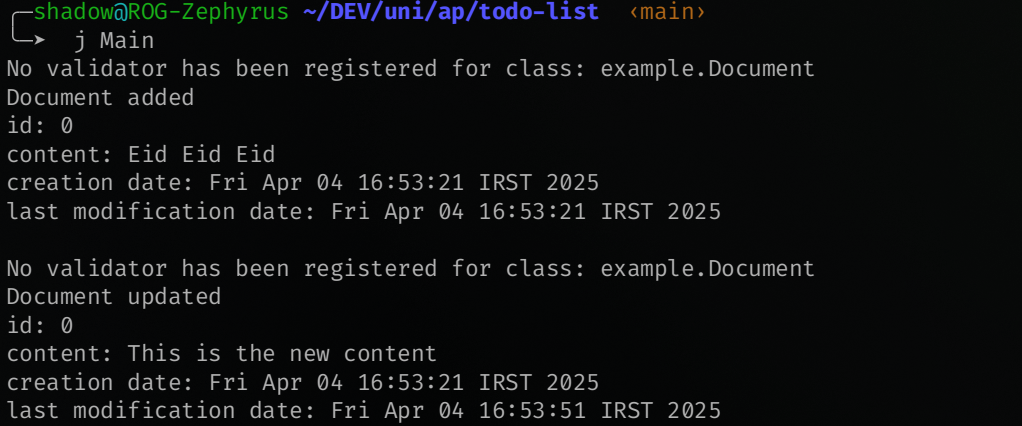
\includegraphics[width=0.8\textwidth]{../img/screenshot3.png}
    \caption*{اسکرین‌شات از خروجی کد حین اجرای بخش تست کد}
\end{figure}

\end{document}